\section{Fits to invariant mass distributions of signal and normalization channel}
\label{sec: massfits}

In order to properly model the invariant mass distribution of $\Bs\to\Ds\kaon\pion\pion$ and $\Bs\to\Ds\pion\pion\pion$ candidates, 
the expected signal shape, as well as the expected shape for the combinatorial and physical background has to be known. 
This model can then be used to fit the distributions and obtain signal sWeights \cite{Pivk:2004ty}, 
which are employed to suppress the residual background that is still left in the sample, for the time-dependent amplitude fit.   

\subsection{Signal models for $\m(\Ds\pion\pion\pion)$ and $m(\Ds\kaon\pion\pion)$}
\label{subsec: signalmodel}

\begin{figure}[h]
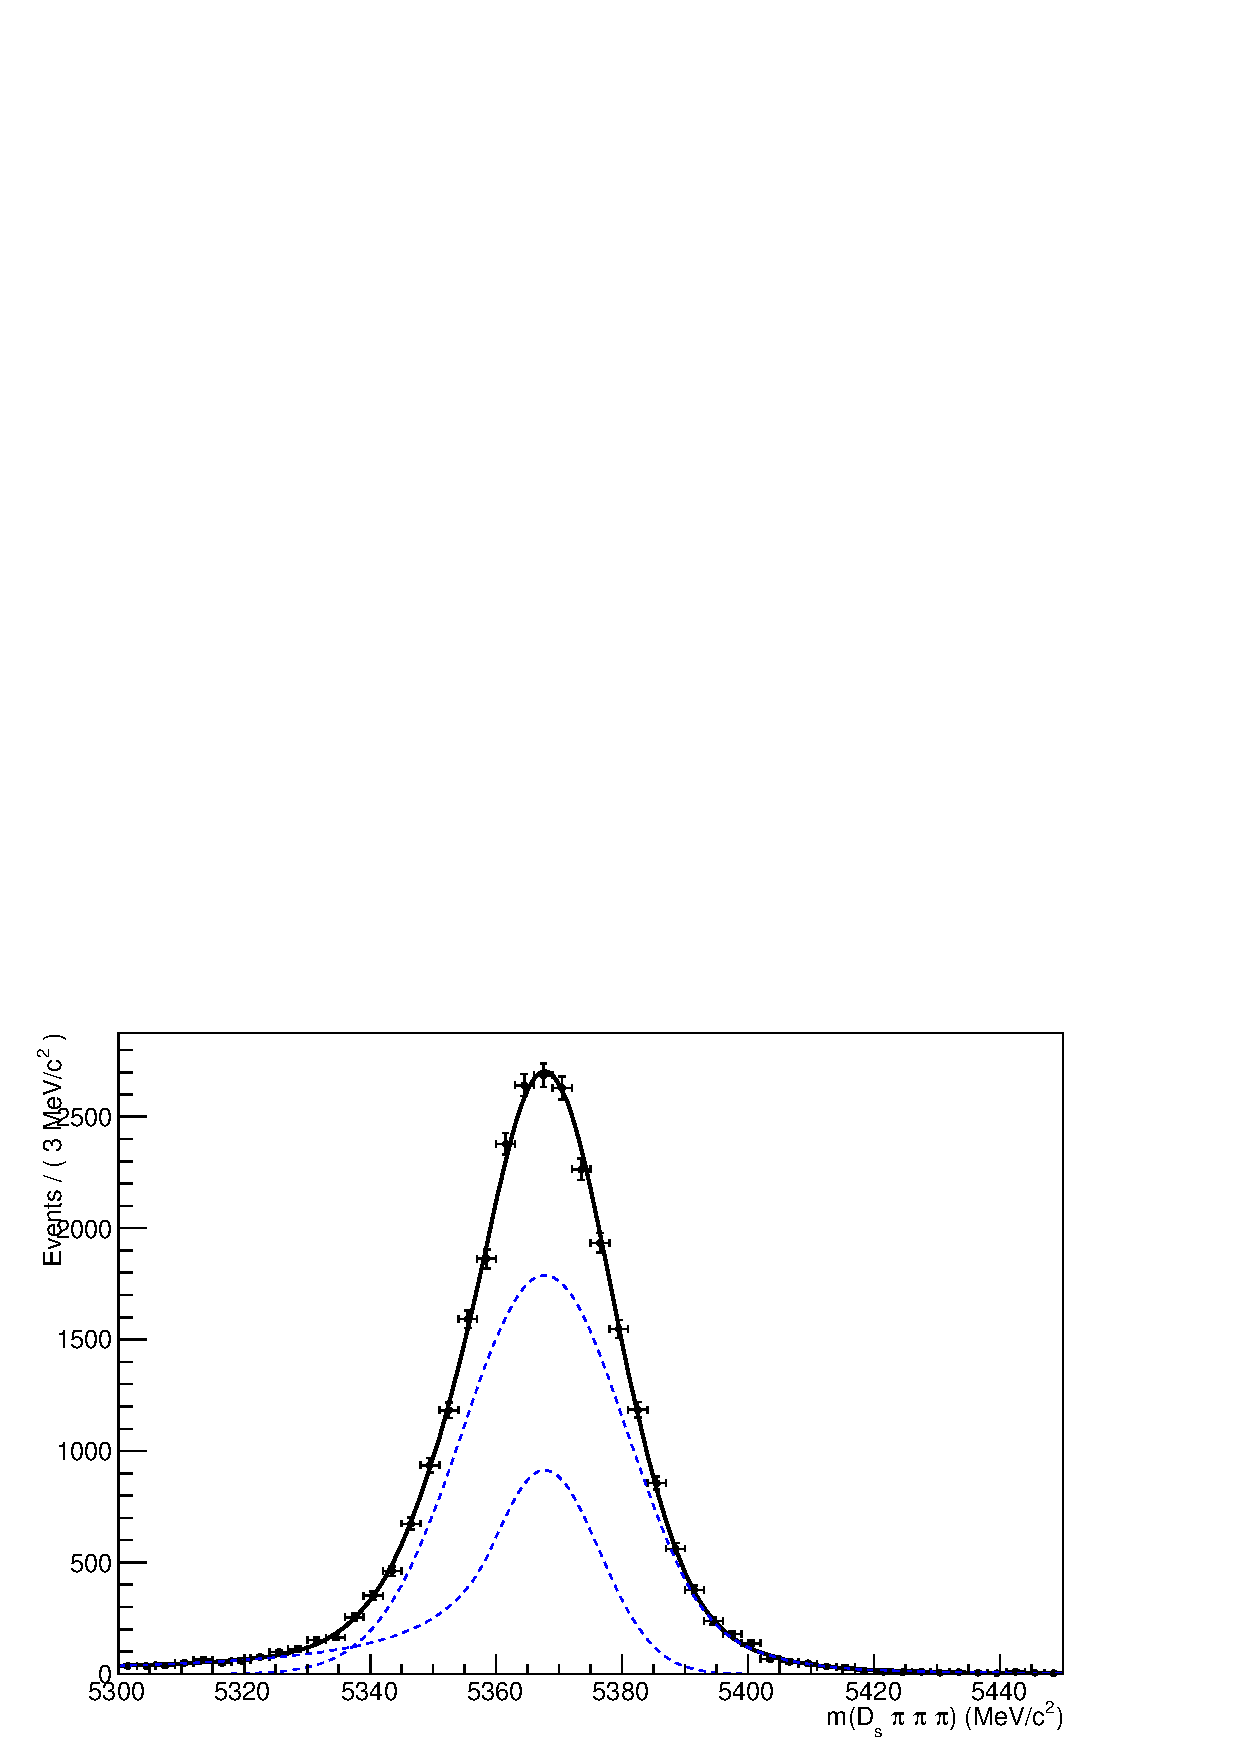
\includegraphics[height=7.cm,width=0.49\textwidth]{figs/Bs2Dspipipi_MC_SignalShape.pdf}
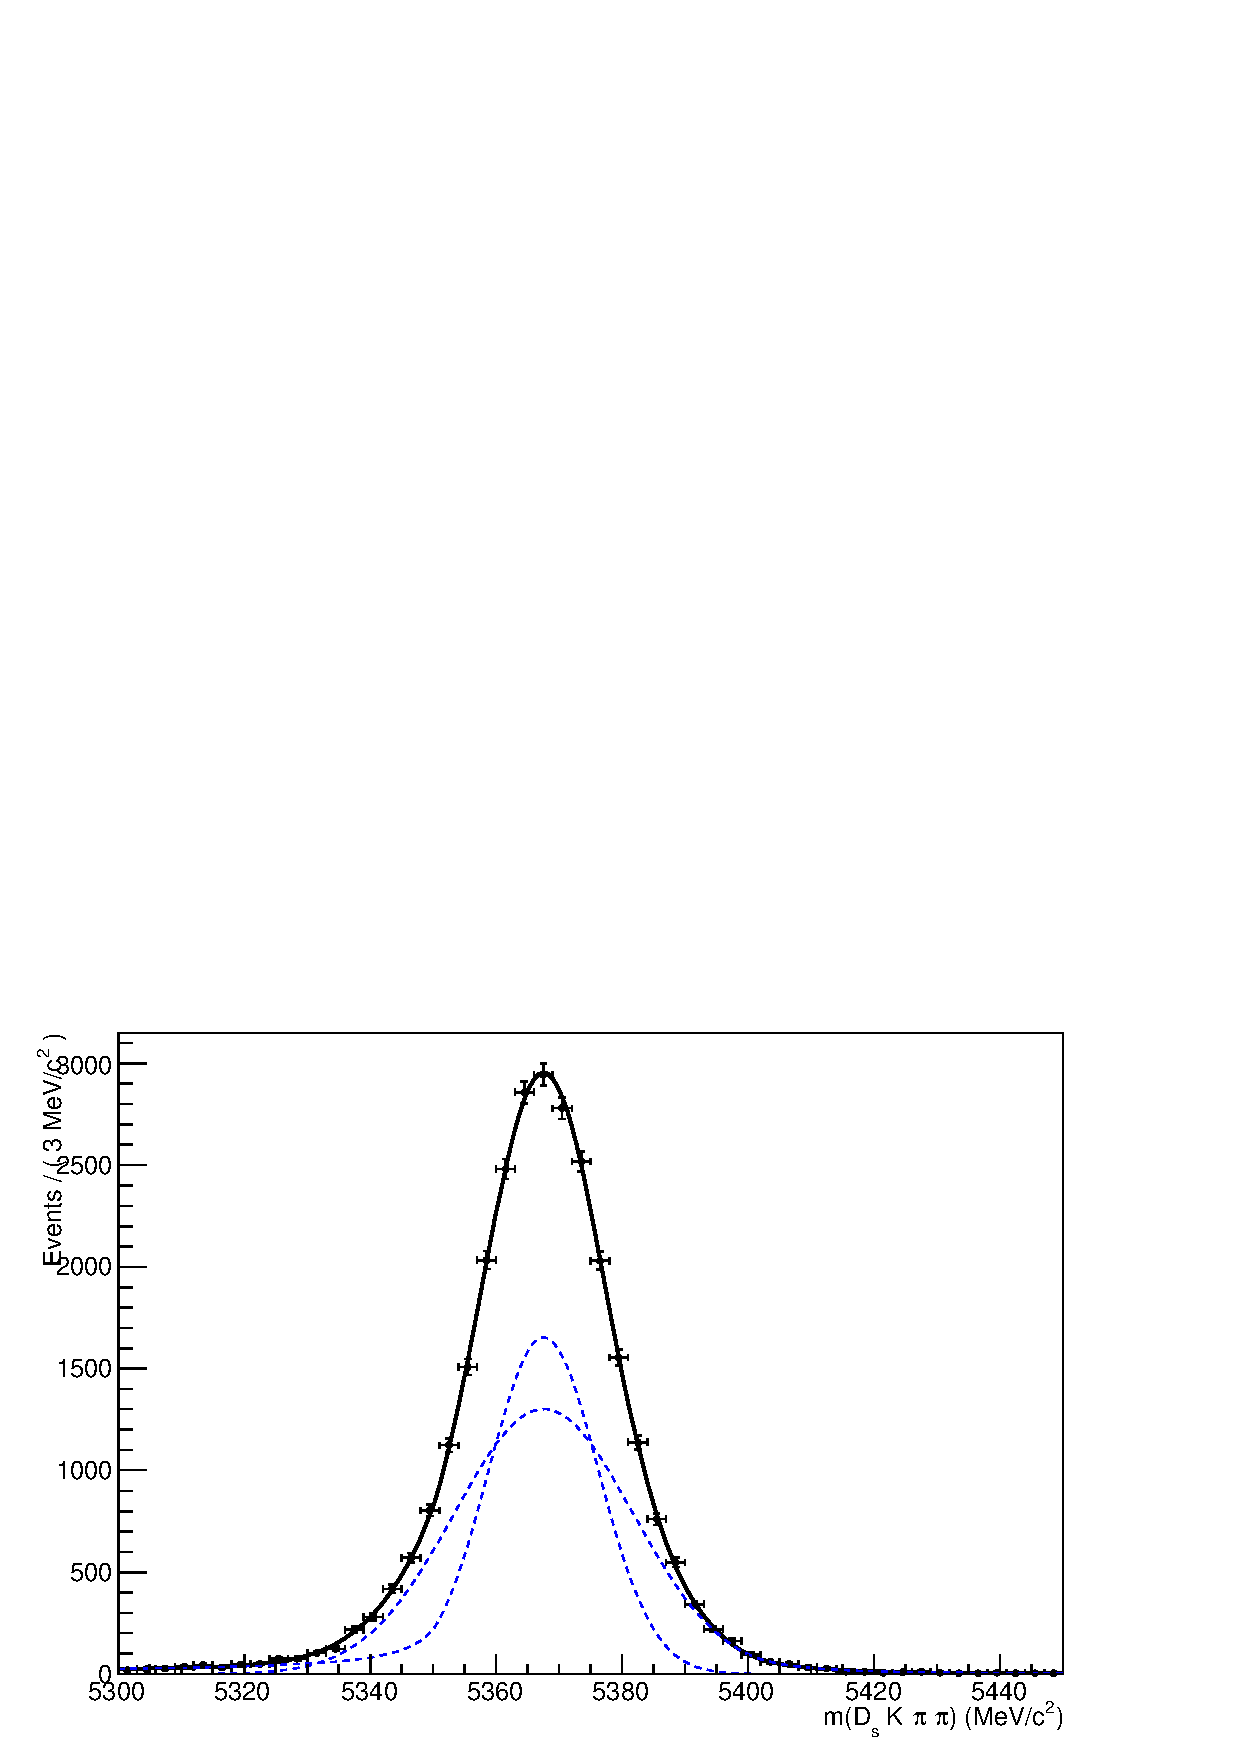
\includegraphics[height=7.cm,width=0.49\textwidth]{figs/Bs2DsKpipi_MC_SignalShape.pdf}
\caption{Invariant mass distributions of simulated (left) $\Bs\to\Ds\pion\pion\pion$ and (right) $\Bs\to\Ds\kaon\pion\pion$ events. A fit of the sum of two Crystal Ball functions to each distribution is overlaid. The dotted lines represent the individual Crystal Ball functions.}
\label{fig: BsMassShapes}
\end{figure}


The mass distribution of $\Bs\to\Ds\kaon\pion\pion$ signals is modeled using two Crystal Ball functions, which share the same mean $\mu$, but are allowed to have different widths $\sigma_{1}$ and $\sigma_{2}$. 
Another double Crystal Ball function is used to account for the contribution of the $\B^{0}\to\Ds\kaon\pion\pion$ decay, which is also present in the $m(\Ds\kaon\pion\pion)$ spectrum.
The core width, as well as the tail parameters and the ratio of the two individual Crsystal Ball functions are fixed to values obtained by a fit to the invariant mass distribution of simulated events shown in Fig \ref{fig: BsMassShapes}. The second width $\sigma_{2}$ and the shared mean $\mu$ are floated in the fit to account for possible differences between the simulation and real data. \newline
The same approach is used to describe the invariant mass distribution of $\Bs\to\Ds\pion\pion\pion$ candidates. 
A double Crystal Ball function is used to model the signal, the parameters are determined by a fit to the invariant mass of simulated $\Bs\to\Ds\pion\pion\pion$ decays, shown in Fig \ref{fig: BsMassShapes}.
The second width and the shared mean are floated to account for differences between data and MC.

\subsection{Background models for $\m(\Ds\pion\pion\pion)$} 
\label{subsec: BkginNorm}
Different background sources arise in the invariant mass spectrum of candidates in the normalization mode. \newline
The following backgrounds have to be accounted for:
\begin{itemize}

\item Combinatorial background: This contribution arises from either a real $\Ds$, which is paired with random tracks to form the $\Bs$ candidates, or via real $X_{d}$'s, which are combined with three tracks that fake a $\Ds$ candidate to form a fake $\Bs$.   

\item Partially reconstructed $\Bs\to\Ds^{*}\pion\pion\pion$ decays, with $\Ds^{*}\to\Ds\gamma$ or $\Ds^{*}\to\Ds\piz$, where the $\gamma$/$\piz$ is not reconstructed in the decay chain. 

\end{itemize}

In both cases of combinatorial background, the distribution in the invariant mass of $\Bs$ candidates is expected to be smooth and decrease with higher masses. 
Therefore, one exponential function is used to model these contributions. \newline
The shape of the  $\Bs\to\Ds^{*}\pion\pion\pion$ contribution is expected to be peaking in the $m(\Ds\pion\pion\pion)$ spectrum, with large tails due to the missing momentum, which is carried away by the $\piz$ or $\gamma$. 
The pion or photon from $\Ds^{*}\to\Ds(\gamma/\piz)$ is excluded from the reconstruction. 
We model the shape of this contribution using the sum of three bifurcated Gaussian functions.
%\begin{figure}[h]
%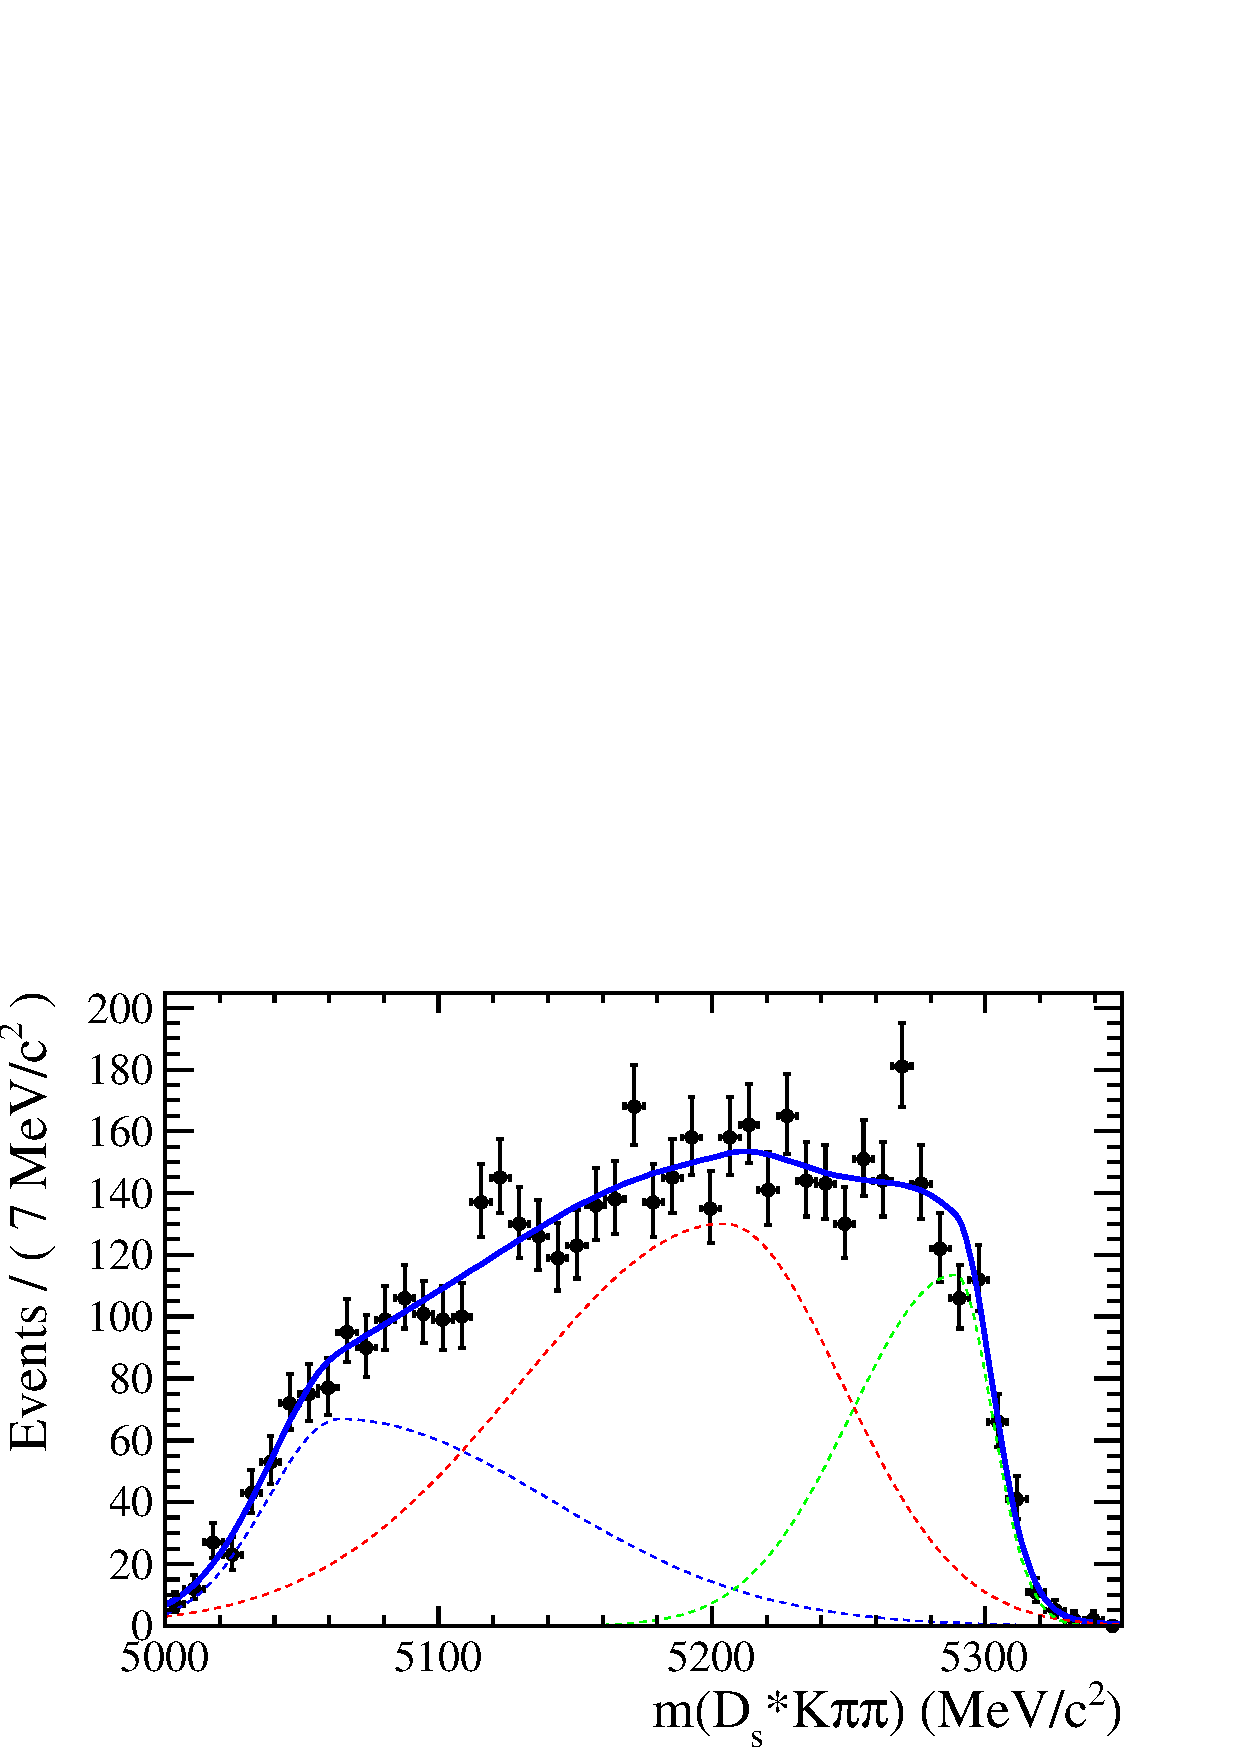
\includegraphics[height=8.cm,width=0.80\textwidth]{figs/Bs2Dsstartpipipi.pdf}
%\caption{Invariant mass distribution of simulated $\Bs\to\Ds^{*}\pion\pion\pion$ events, where the $\gamma$/$\piz$ is excluded from the reconstruction. 
%A fit of the sum of three bifurcated Gaussian functions to this distribution is overlaid.}
%\label{fig: BsDsstar3piMC}
%\end{figure}
%Figure \ref{fig: BsDsstar3piMC} shows the fit of the sum of three bifurcated Gaussian functions to the invariant mass distribution of simulated $\Bs\to\Ds^{*}\pion\pion\pion$ event. 
The shape parameters, 
%are used as input values for the nominal $m(\Ds\pion\pion\pion)$ mass fit. 
as well as the yield of this contribution, are directly determined on data from a fit to the $m(\Ds\pion\pion\pion)$ invariant mass distribution. 

\subsection{Background models for $m(\Ds\kaon\pion\pion)$}
For the signal channel, the following background sources have to be considered:

\begin{itemize}

\item Combinatorial background: same contributions as discussed in Sec. \ref{subsec: BkginNorm}.

\item Partially reconstructed $\Bs\to\Ds^{*}\kaon\pion\pion$ decays, with $\Ds^{*}\to\Ds\gamma$ or $\Ds^{*}\to\Ds\piz$, where the $\gamma$/$\piz$ is not reconstructed in the decay chain. 

\item Partially reconstructed $\Bz\to\Ds^{*}\kaon\pion\pion$ decays, with $\Ds^{*}\to\Ds\gamma$ or $\Ds^{*}\to\Ds\piz$, where the $\gamma$/$\piz$ is not reconstructed in the decay chain.

\item Misidentified $\Bs\to\Ds\pion\pion\pion$ decays, where one of the pions is wrongly identified as a kaon $\pion\rightarrow\kaon$.  

\item Misidentified, partially reconstructed $\Bs\to\Ds^{*}\pion\pion\pion$ decays, where one of the pions is wrongly identified as a kaon $\pion\rightarrow\kaon$ and the $\gamma$/$\piz$ from $\Ds^{*}\to\Ds\gamma$/$\piz$ is 
not reconstructed.

\end{itemize}

The combinatorial background is expected to be non-peaking in the spectrum of the invariant mass of $\Bs\to\Ds\kaon\pion\pion$ candidates. An exponential function is used to model this contribution.\newline
The shape of the partially reconstructed background without misID is taken from our normalization channel, where it can be directly fitted by the sum of three bifurcated Gaussian functions as described above.
In the signal mass fit, all shape parameters for the $\Bs\to\Ds^{*}\kaon\pion\pion$ background are fixed to the input values from our normalization fit.  
%A MC sample of $\Bs\to\Ds^{*}\kaon\pion\pion$ events, where the $\gamma$/$\piz$ is excluded from the reconstruction, is generated. 
%The sum of three bifurcated gaussians is then fitted to the mass distribution of $\Bs$ candidates. The distribution and the overlaid fit is shown in Fig. \ref{fig: BsDsstarKpipiMC}.  

%\begin{figure}[h]
%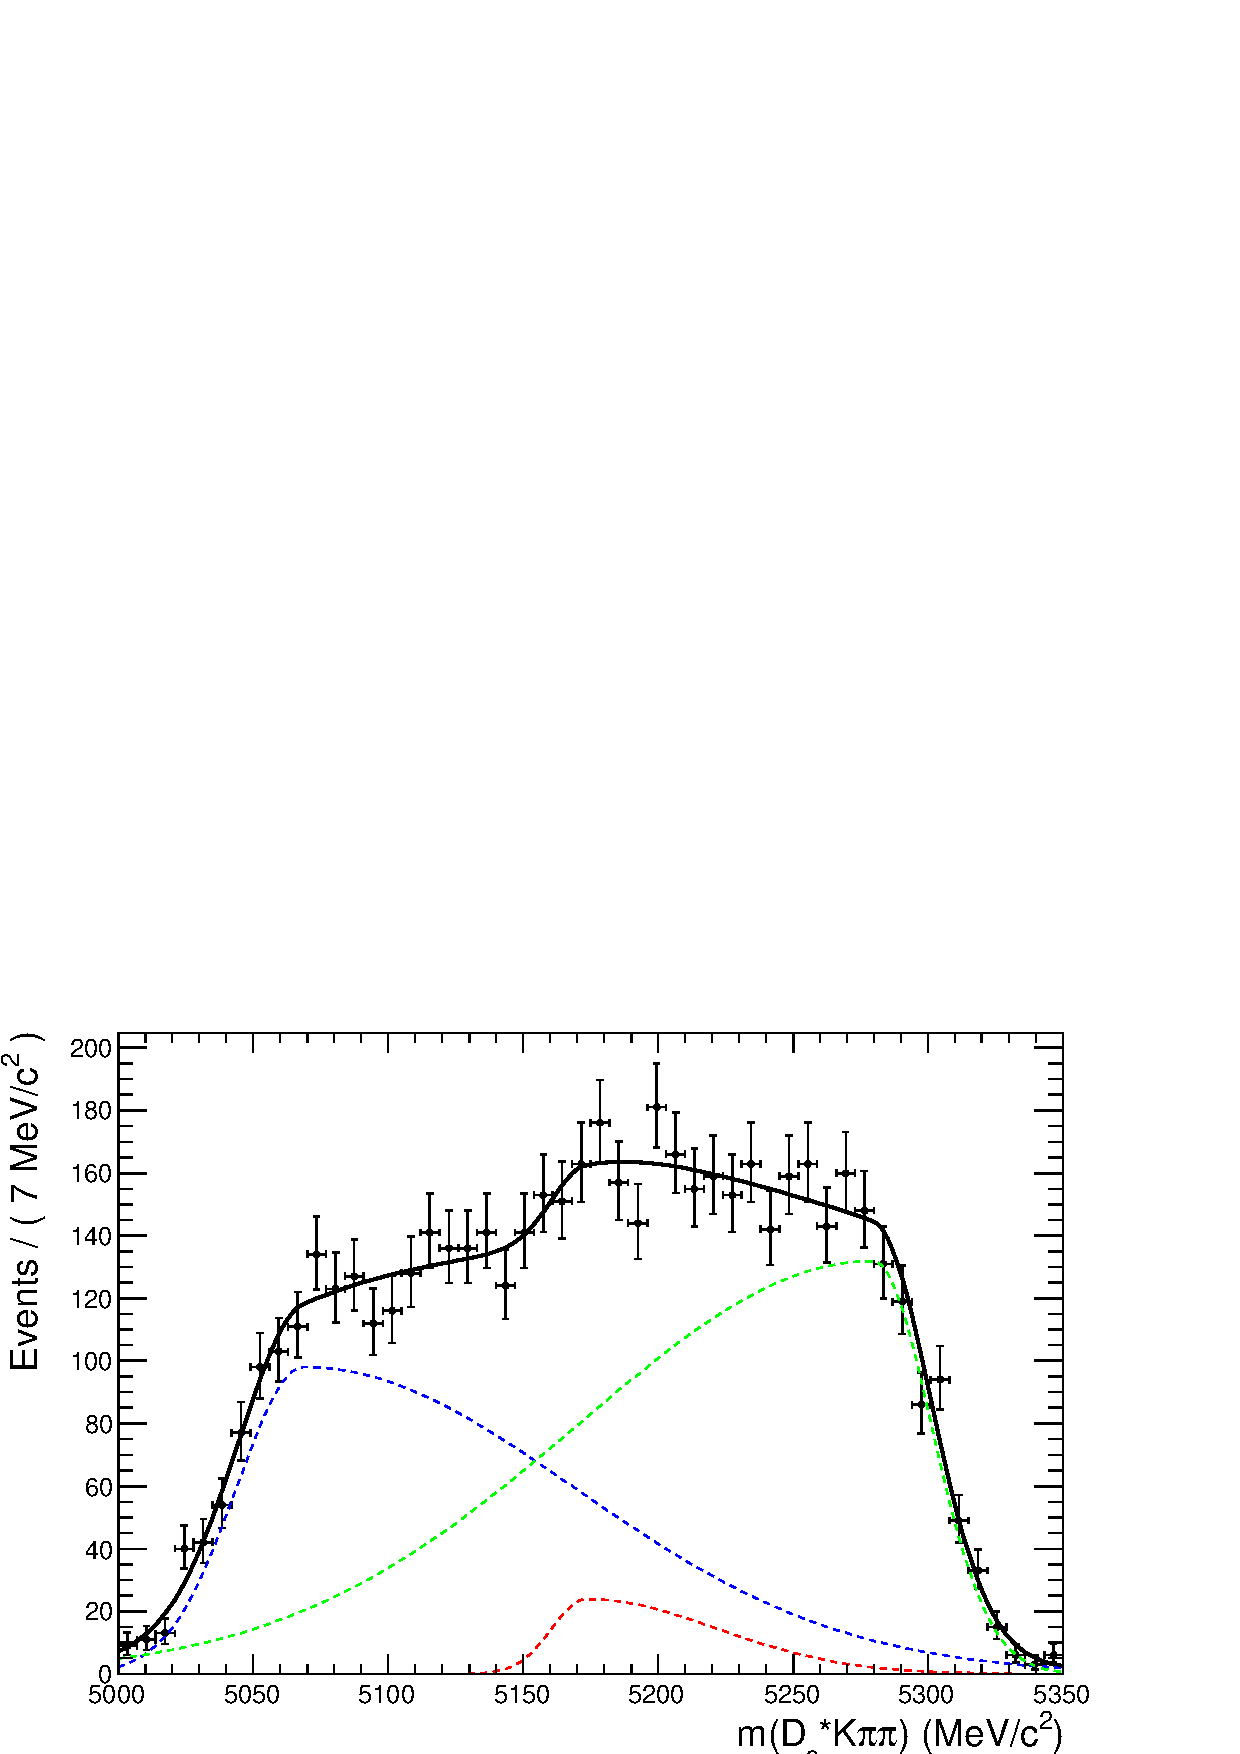
\includegraphics[height=8.cm,width=0.80\textwidth]{figs/Bs2DsstartKpipi.pdf}
%\caption{Invariant mass distribution of simulated $\Bs\to\Ds^{*}\kaon\pion\pion$ events, where the $\gamma$/$\piz$ is excluded from the reconstruction. 
%A fit of the sum of three bifurcated gaussians to this distribution is overlaid.}
%\label{fig: BsDsstarKpipiMC}
%\end{figure}

For the contribution of the $\Bz\to\Ds^{*}\kaon\pion\pion$ background, the same shape is used but the means $\mu_{i}$ of the bifurcated gaussians are shifted down by $m_{\Bs} - m_{\Bz}$ \cite{Agashe:2014kda}. 
The yields of both contributions are directly determined in the nominal fit. \newline
To determine the shape of misidentified $\Bs\to\Ds\pion\pion\pion$ candidates in the $m(\Ds\kaon\pion\pion)$ spectrum, we take a truth-matched signal MC sample of our normalization channel. 
We then use the PIDCalib package to determine the $\pion\rightarrow\kaon$ fake rate. For every candidate in our MC sample, a (momentum) $\ptot$ and (pseudorapidity) $\eta$-dependent event weight is computed and assigned. 
We flip the particle hypothesis from pion to kaon for the $\pion$ with the biggest miss-ID weight for each event and recompute the invariant $\Bs$ mass. This distribution is then modeled using two Crystal Ball functions. 
The distribution and the fit are shown in Fig. \ref{fig: BsDspipipiMCmissID}(left). 

\begin{figure}[h]
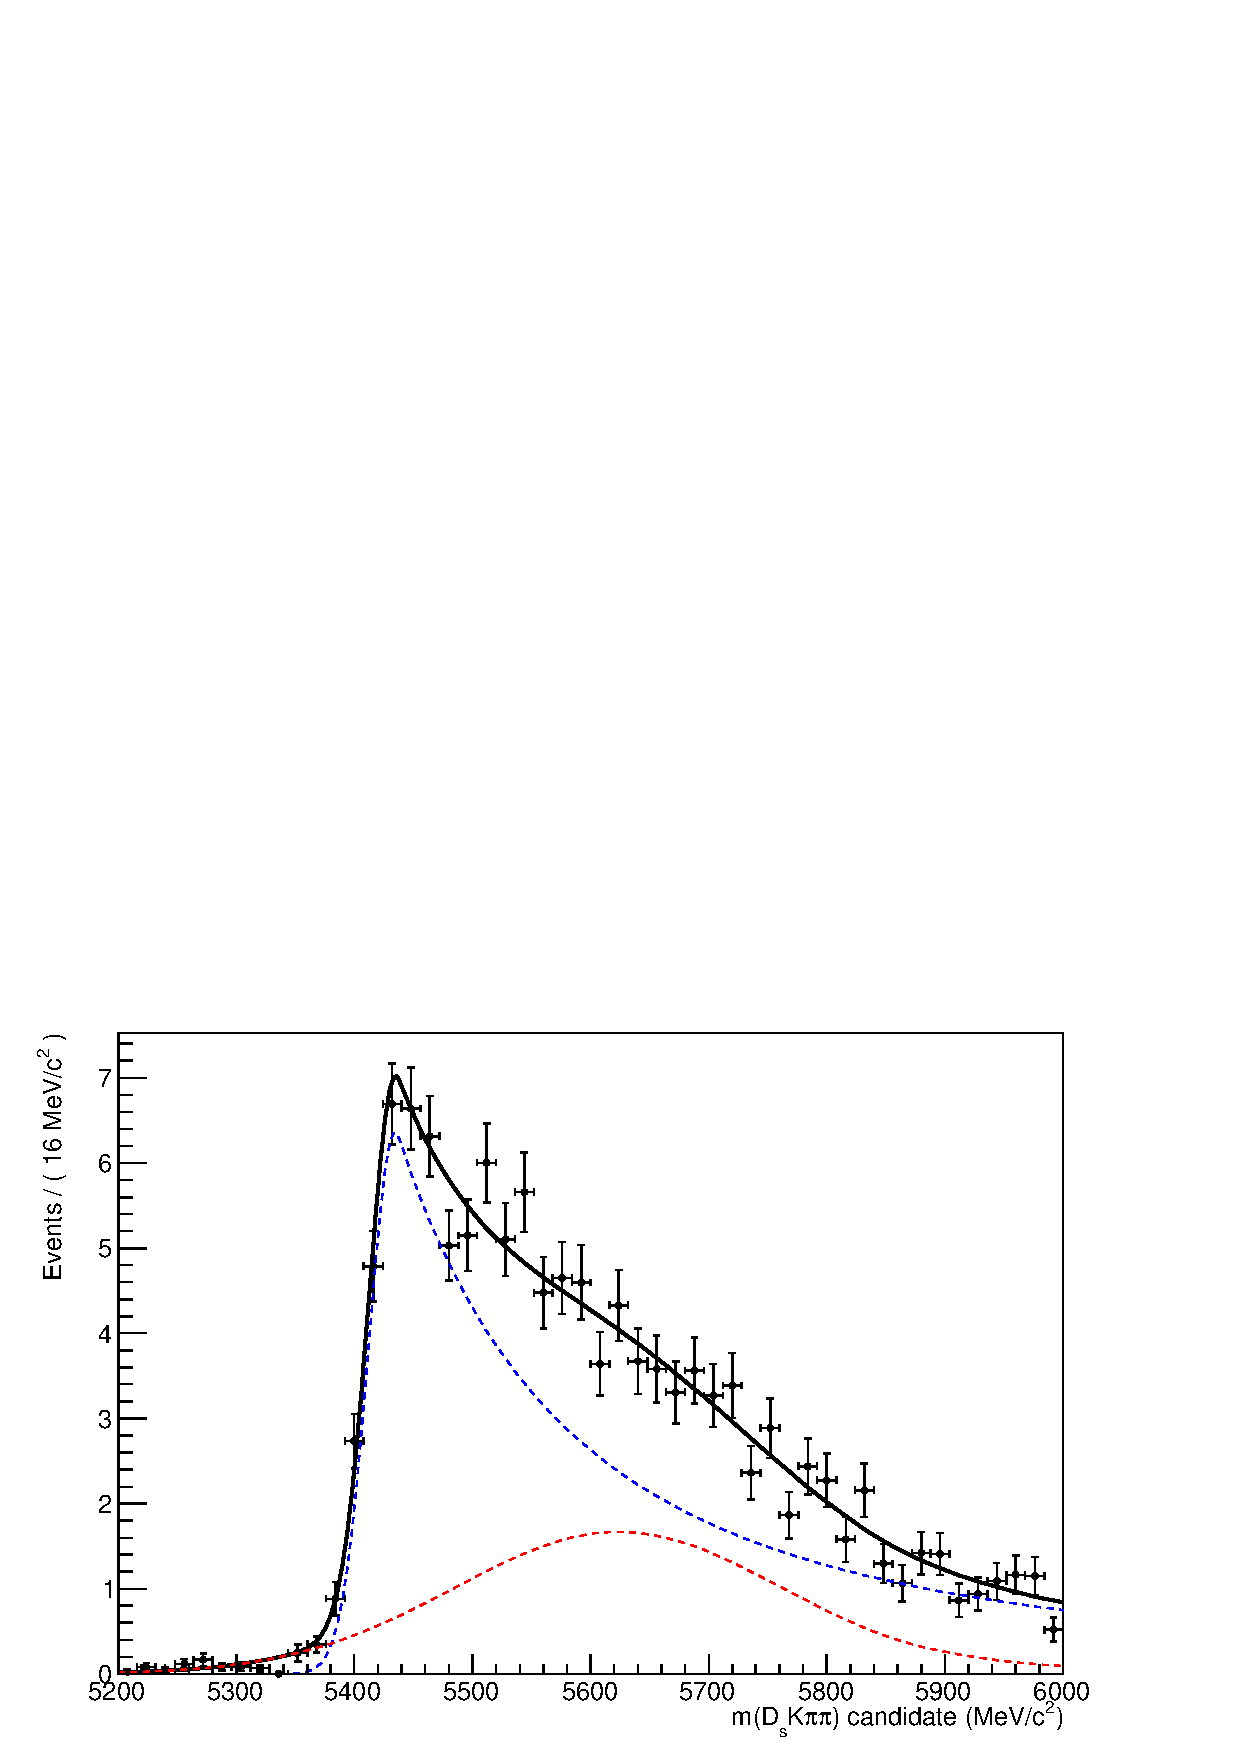
\includegraphics[height=6.cm,width=0.45\textwidth]{figs/Bs2Dspipipi_as_DsKpipi.pdf}
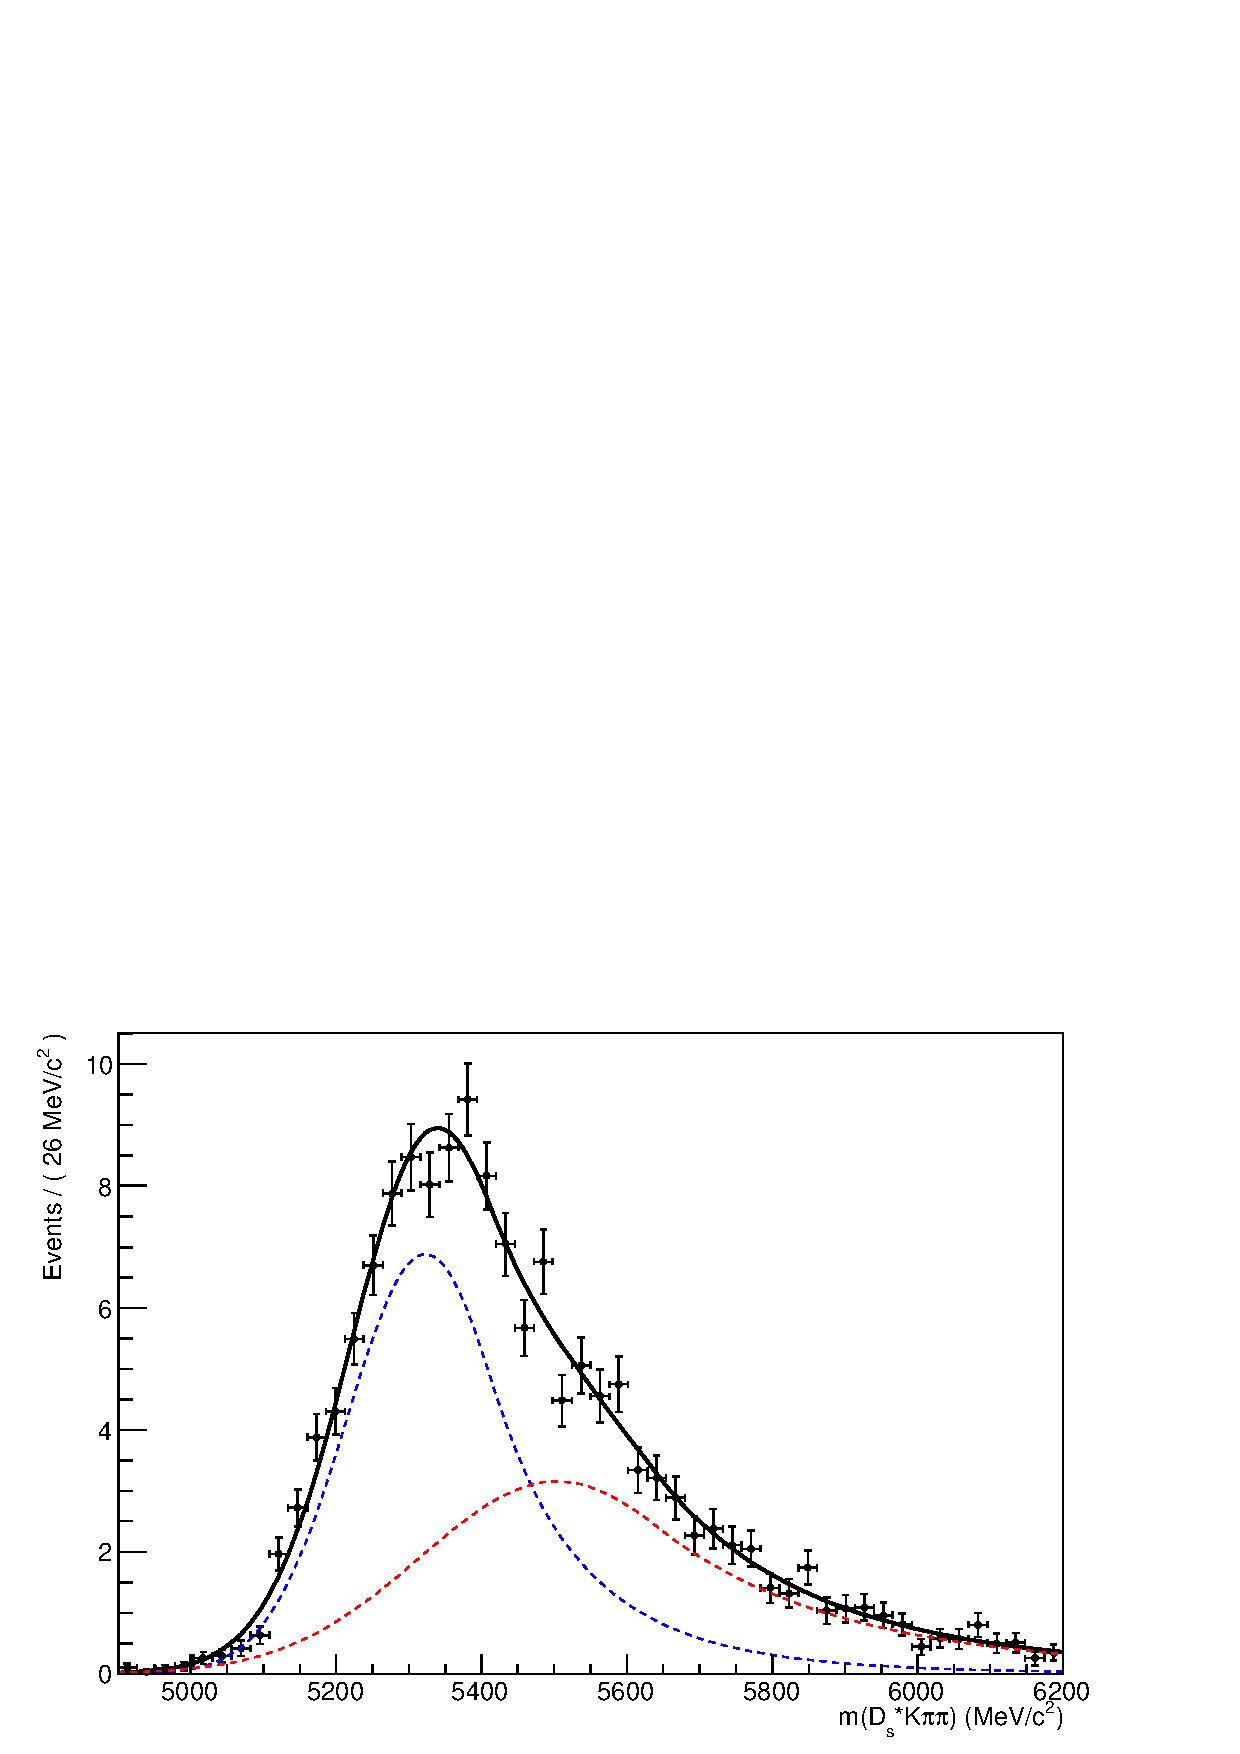
\includegraphics[height=6.cm,width=0.45\textwidth]{figs/Bs2Dsstarpipipi_as_DsKpipi.pdf}
\caption{Invariant mass distribution of (left) simulated $\Bs\to\Ds\pion\pion\pion$ events, where one of the $\pion$'s is reconstructed as a $\kaon$ and the misID probability for each event is taken into account. 
The corresponding distribution for simulated $\Bs\to\Ds^{*}\pion\pion\pion$ events, where the $\gamma$/$\piz$ from the $\Ds^{*}$ is excluded from reconstruction, is shown on the right.
The solid, black curve on each plot corresponds to the fit consisting of two Crystal Ball functions.}
\label{fig: BsDspipipiMCmissID}
\end{figure}
 
The expected yield of misidentified $\Bs\to\Ds\pion\pion\pion$ candidates in the $m(\Ds\kaon\pion\pion)$ spectrum is computed by multiplying the fake probability of $\propto3.2\%$, which is derived from PIDCalib, by the yield of $\Bs\to\Ds\pion\pion\pion$ signal candidates, determined in the nominal mass fit of our normalization channel.  \newline
In the same way as mentioned above, we can determine the rate of misidentified, partially reconstructed $\Bs\to\Ds^{*}\pion\pion\pion$ decays in our sample of $\Bs\to\Ds\kaon\pion\pion$ decays using PIDCalib and a MC sample of $\Bs\to\Ds^{*}\pion\pion\pion$ events. The invariant mass distribution we obtain when we exclude the $\gamma$/$\piz$, flip the the particle hypothesis $\pion\rightarrow\kaon$ and apply the event weights given by the fake rate, is shown in Fig. \ref{fig: BsDspipipiMCmissID} (right). The fit of two Crystal Ball functions to this distribution is overlaid. 
The yield of this contribution is determined from the yield of $\Bs\to\Ds^{*}\pion\pion\pion$ candidates in the nominal mass fit of our normalization channel, multiplied by the misID probability of $\propto 3.6\%$.
 



\subsection{Fit to $\Bs\to\Ds\pion\pion\pion$ candidates}
\label{subsec: NormFit}

An unbinned maximum likelihood fit is performed simultaneously to the invariant mass distribution of $\Bs\to\Ds\pion\pion\pion$ candidates. 
As discussed in Sec. \ref{subsec: signalmodel}, the fit is given as the sum of the double Gaussian signal model, the sum of three bifurcated Gaussian functions to model the partially reconstructed $\Bs\to\Ds^{*}\pion\pion\pion$ background and an Exponential function to account for combinatorial background. The invariant mass distribution and the fit is shown in Fig. \ref{fig: BsDsKpipiFit}. 
The obtained yields are summarized in Tab. \ref{tab: SigYields}.

%The determined number of $\Bs\to\Ds\pion\pion\pion$ decays is $8496 \pm 102$ for 2011 data and $19410 \pm 160$ for 2012 data. 
%The determined yield for the partially reconstructed $\Bs\to\Ds^{*}\pion\pion\pion$ background is  (2011) $16904 \pm 299$ and (2012)  $38437 \pm 589$, 
%while the yield for the combinatorial background is (2011) $16066 \pm 304$ and (2012) $35285 \pm 596$.



\subsection{Fit to $\Bs\to\Ds\kaon\pion\pion$ candidates}
\label{subsec: SigFit}

The shape of the invariant mass distribution of$\Bs\to\Ds\kaon\pion\pion$ candidates is described by the sum of two double Gaussian functions for the $\Bz$ and $\Bs$ signal, 
two sums of three bifurcated Gaussians for the $\Bs$/$\Bz\to\Ds^{*}\kaon\pion\pion$ partially reconstructed background contributions and 
two sums of double Crystal Ball functions for the single misID $\Bs\to\Ds\pion\pion\pion$ and the partially reconstructed, misidentified $\Bs\to\Ds^{*}\pion\pion\pion$ decays. 
A simultaneous unbinned maximum likelihood fit is performed and the result is shown in Fig. \ref{fig: BsDsKpipiFit}.
The obtained yields are summarized in Tab. \ref{tab: SigYields}.
 

\subsection{Extraction of signal weights}
\label{subsec: sWegihts}

The sPlot technique \cite{Pivk:2004ty} is used to extract signal weights from the fits to the invariant mass distributions of our signal and normalizaton channel. 
This statistical tool assignes a weight to every event, according to it's position in the respective mass distribution, given the fitted signal and background models. 
The weights can then be used to suppress the background components in every other observable distribution of interest.  
Figure \ref{fig: sWeights} shows the distribution of weights across the invariant mass spectra of $\Bs\to\Ds\pion\pion\pion$ and $\Bs\to\Ds\kaon\pion\pion$ candidates.


\begin{figure}[h]
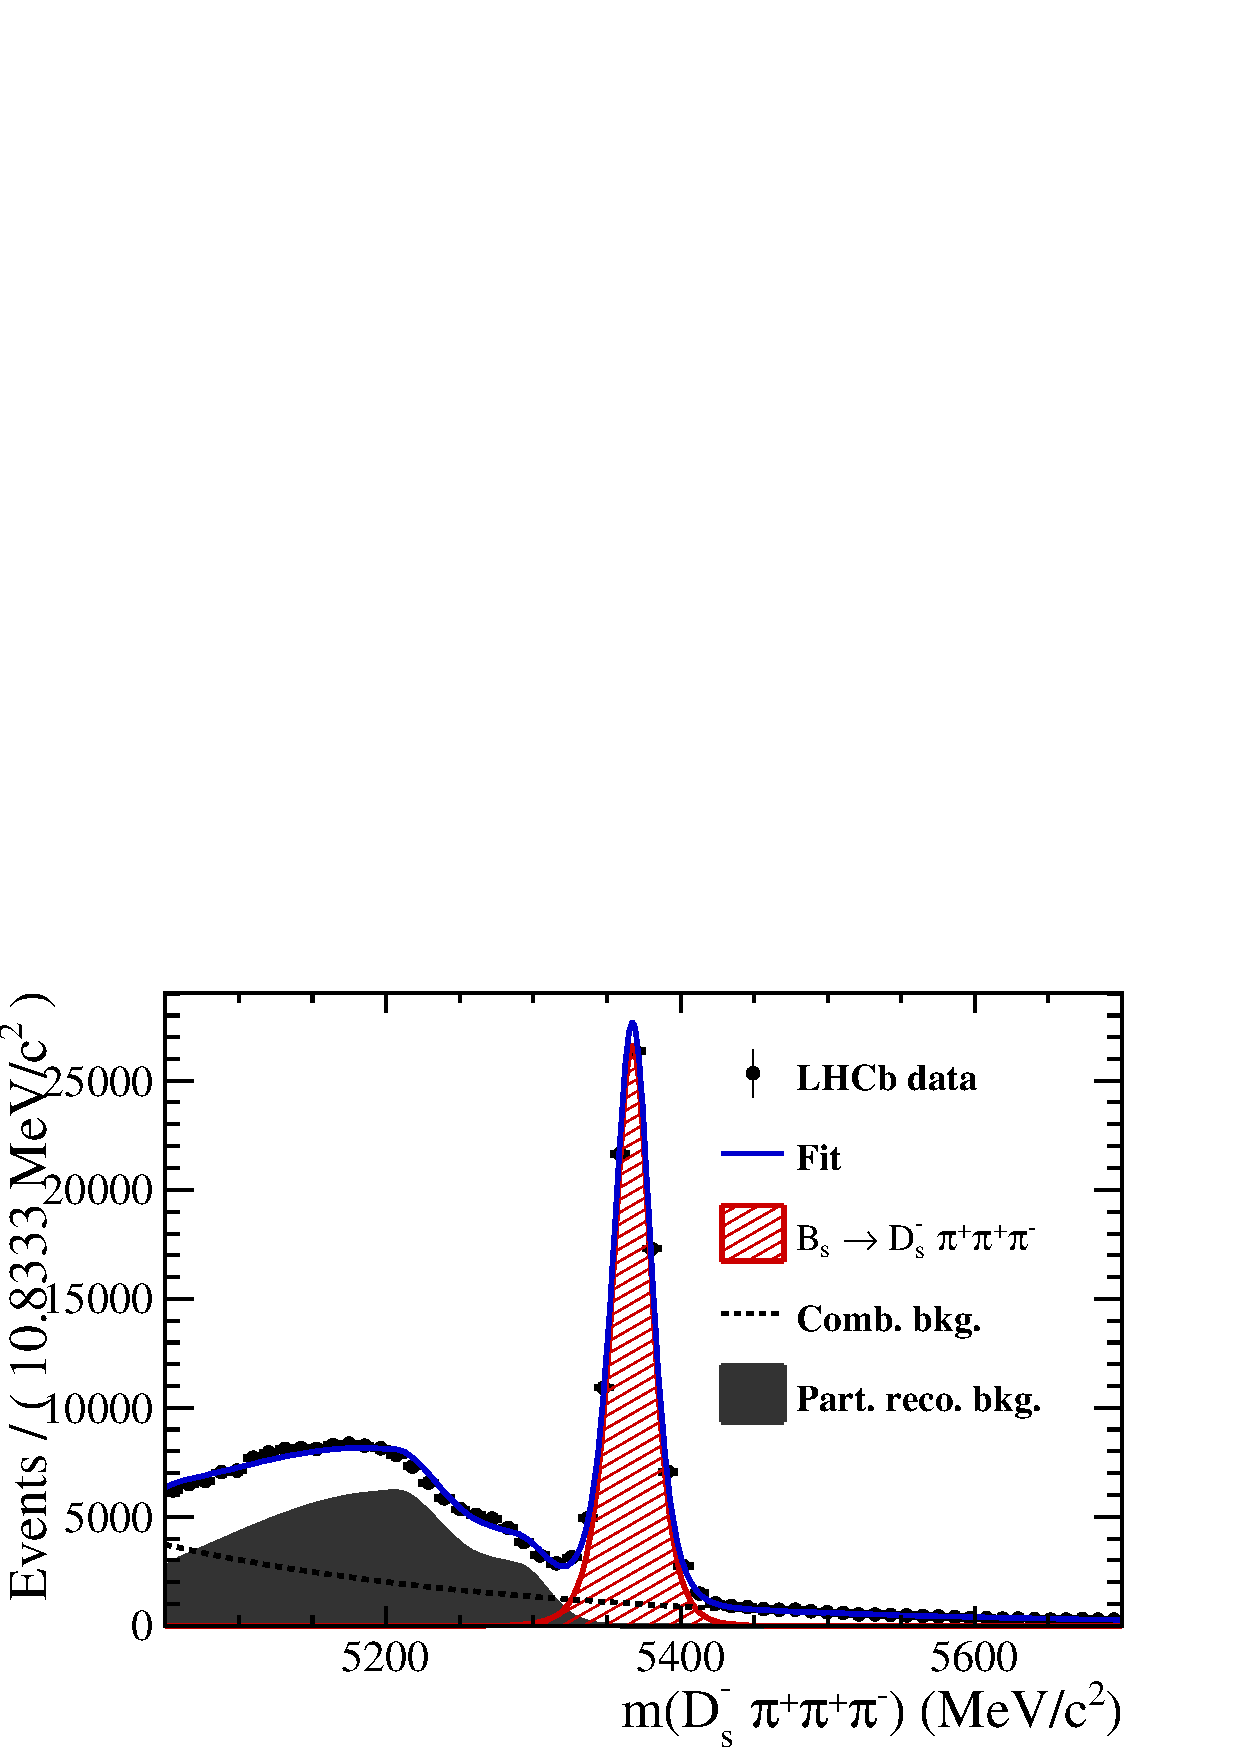
\includegraphics[height=7.cm,width=0.49\textwidth]{figs/norm.pdf}
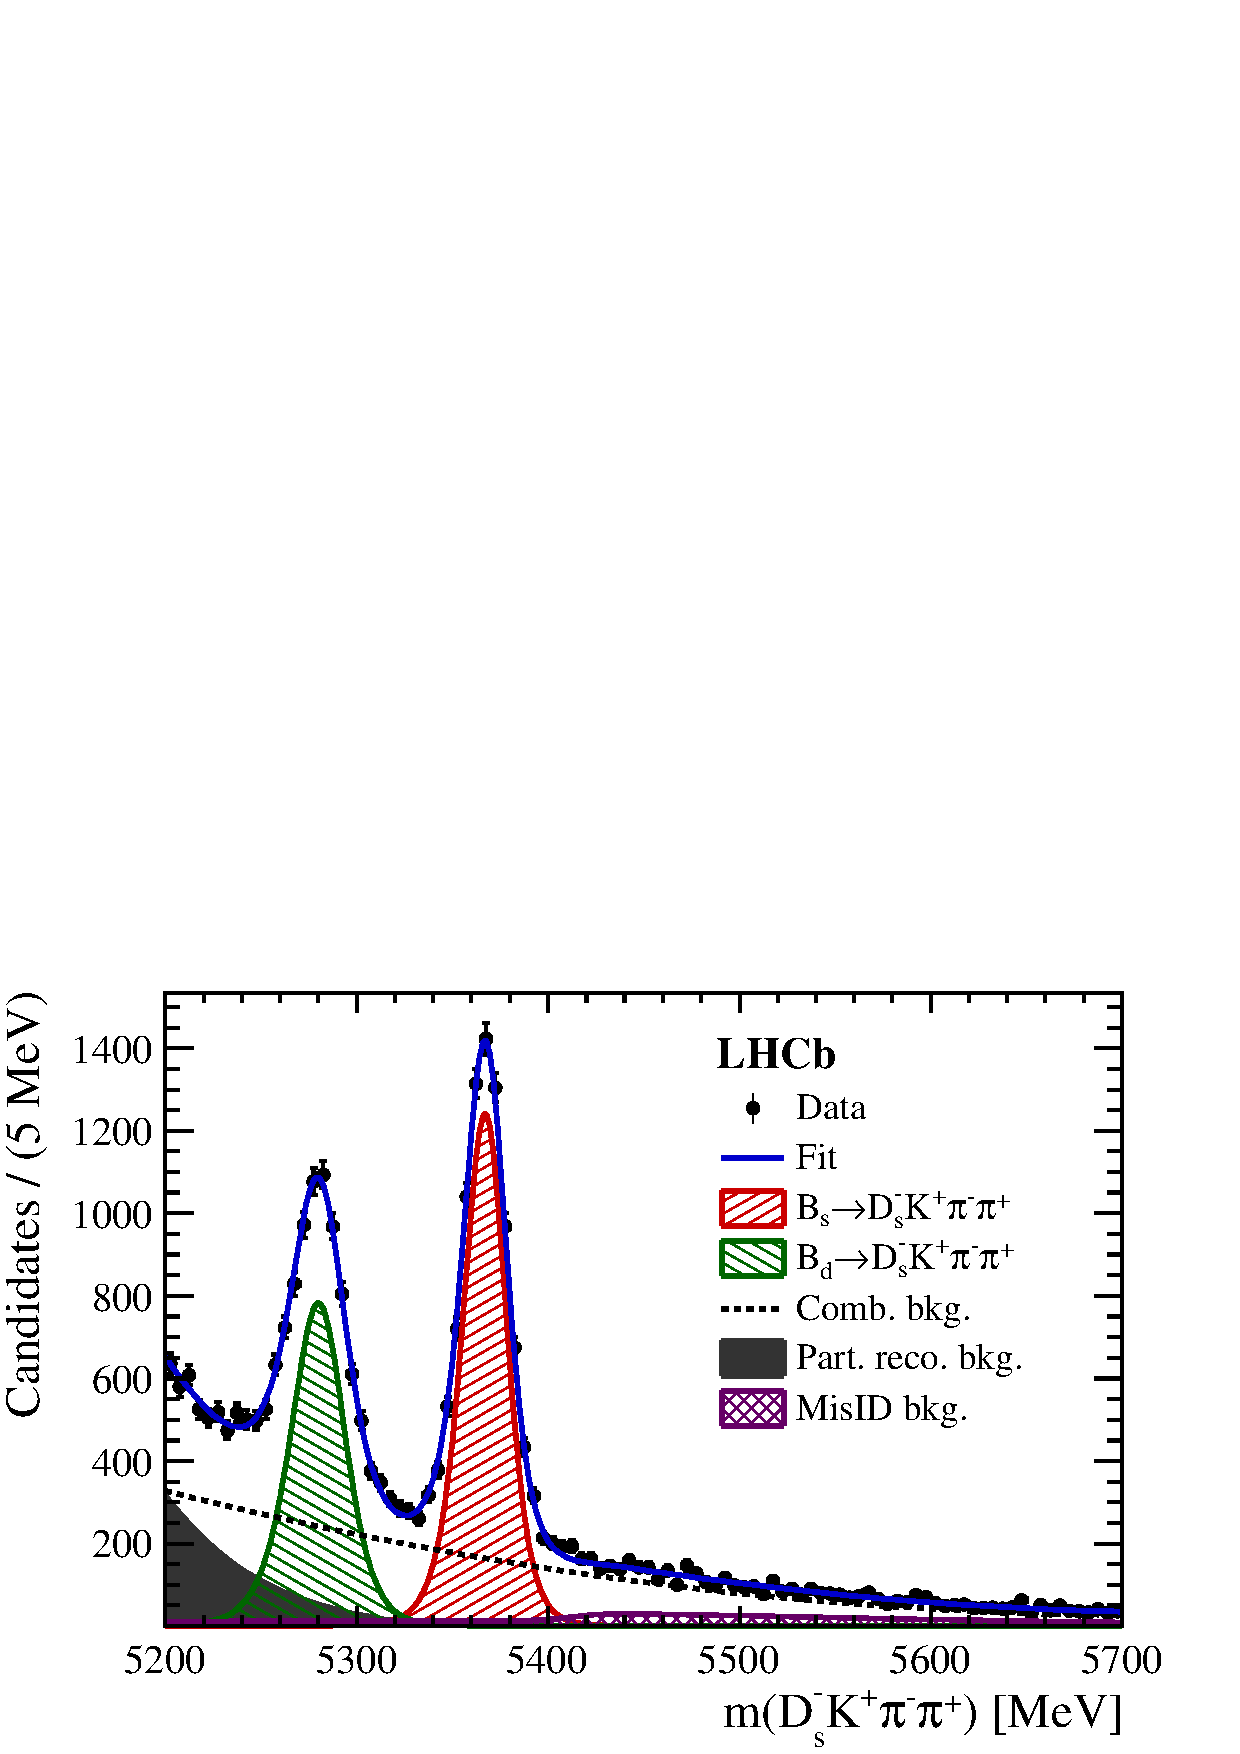
\includegraphics[height=7.cm,width=0.49\textwidth]{figs/signal.pdf}\\
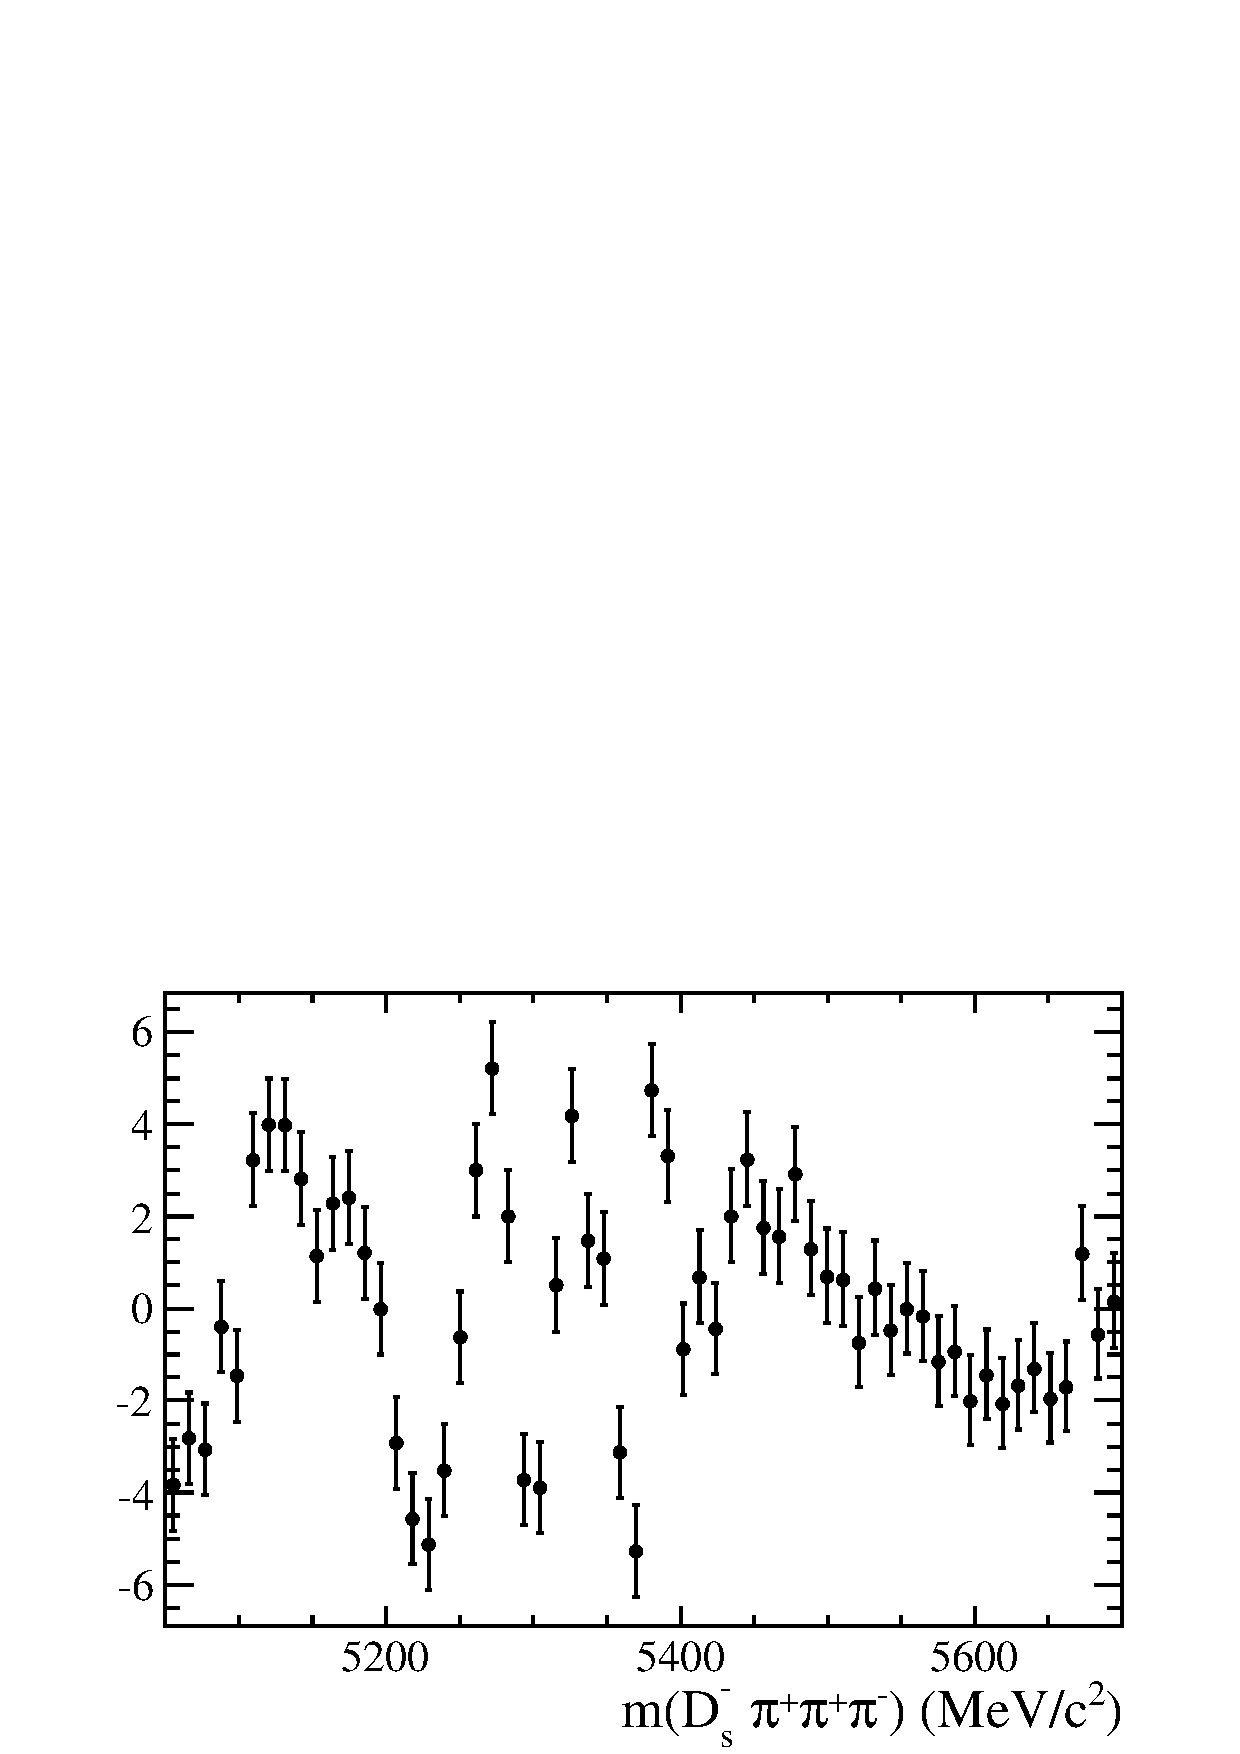
\includegraphics[width=0.49\textwidth,height=1.5cm]{figs/norm_pull.pdf}
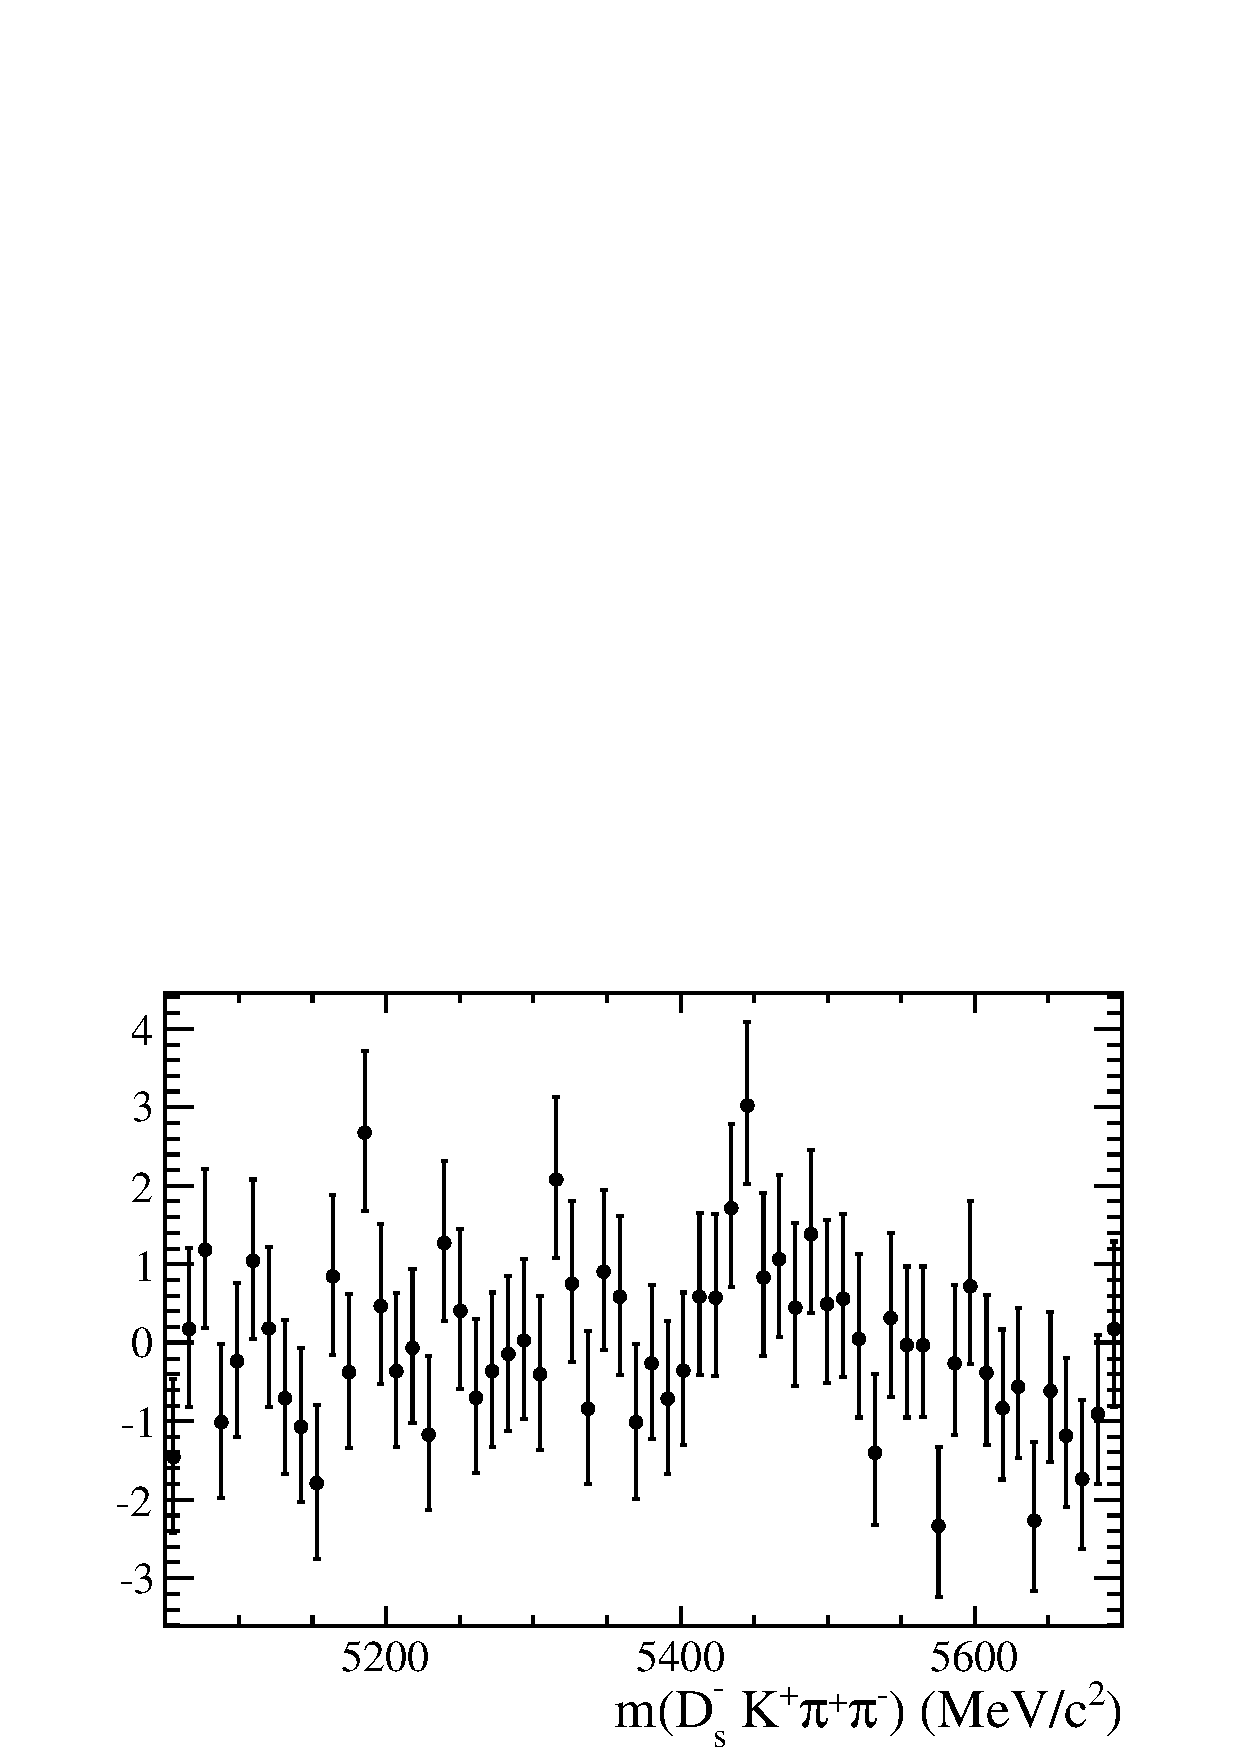
\includegraphics[width=0.49\textwidth,height=1.5cm]{figs/signal_pull.pdf}
\caption{Invariant mass distribution of (left) $\Bs\to\Ds\pion\pion\pion$ and (right) $\Bs\to\Ds\kaon\pion\pion$ candidates for Run1 and Run2 data.
The respective fit described in the text is overlaid.} %The dashed lines show the (magenta) partially reconstructed and (red) combinatorial background, as well as the (blue) signal component. 
%The dashed green line depicts the misID backgrounds and the dashed yellow line depicts the misidentified, partially reconstructed background component. 
%The pull distributions for the simultaneous fit are shown at the lower left and right.}
\label{fig: BsDsKpipiFit}
\end{figure}


\begin{table}[h]
\centering
\begin{tabular}{l c c c c}
invariant mass spectrum/fit component & yield 2011 & yield 2012  & yield 2015  & yield 2016\\
\hline \hline
$m(\Ds\kaon\pion\pion)$    &                  &       &           &\\
\hline
$\Bs\to\Ds\kaon\pion\pion$    &  $351 \pm 26$    &  $858 \pm 40$ & &\\
$\Bz\to\Ds\kaon\pion\pion$    &  $821 \pm 41$    &  $1721 \pm 67$ & &\\
$\Bs\to\Ds^{*}\kaon\pion\pion$ &  $629 \pm 68$   &  $1333 \pm 129$ & &\\
$\Bz\to\Ds^{*}\kaon\pion\pion$ &  $1252 \pm 188$ &  $2653 \pm 400$ & &\\
$\Bs\to\Ds\pion\pion\pion$    &  $257$ (fixed)   & $582$ (fixed & &)\\
$\Bs\to\Ds^{*}\pion\pion\pion$ &  $359$ (fixed)  & $845$ (fixed) & &\\
combinatorial                 &  $2999 \pm 154$  & $6689 \pm 240$ & &\\
\hline \hline
$m(\Ds\pion\pion\pion)$       &                  &    &           & \\
\hline
$\Bs\to\Ds\pion\pion\pion$    &  $7671 \pm 96$  &  $17379 \pm 148$ & &\\
$\Bs\to\Ds^{*}\pion\pion\pion$ & $9984 \pm 193$  & $23479 \pm 357$ & &\\
combinatorial                 & $10341 \pm 204$  & $21737 \pm 373$ & &\\
\hline
\end{tabular}
\caption{Summary of yields from the fits to Run1 and Run2 data.}
\label{tab: SigYields}
\end{table}



\begin{figure}[h]
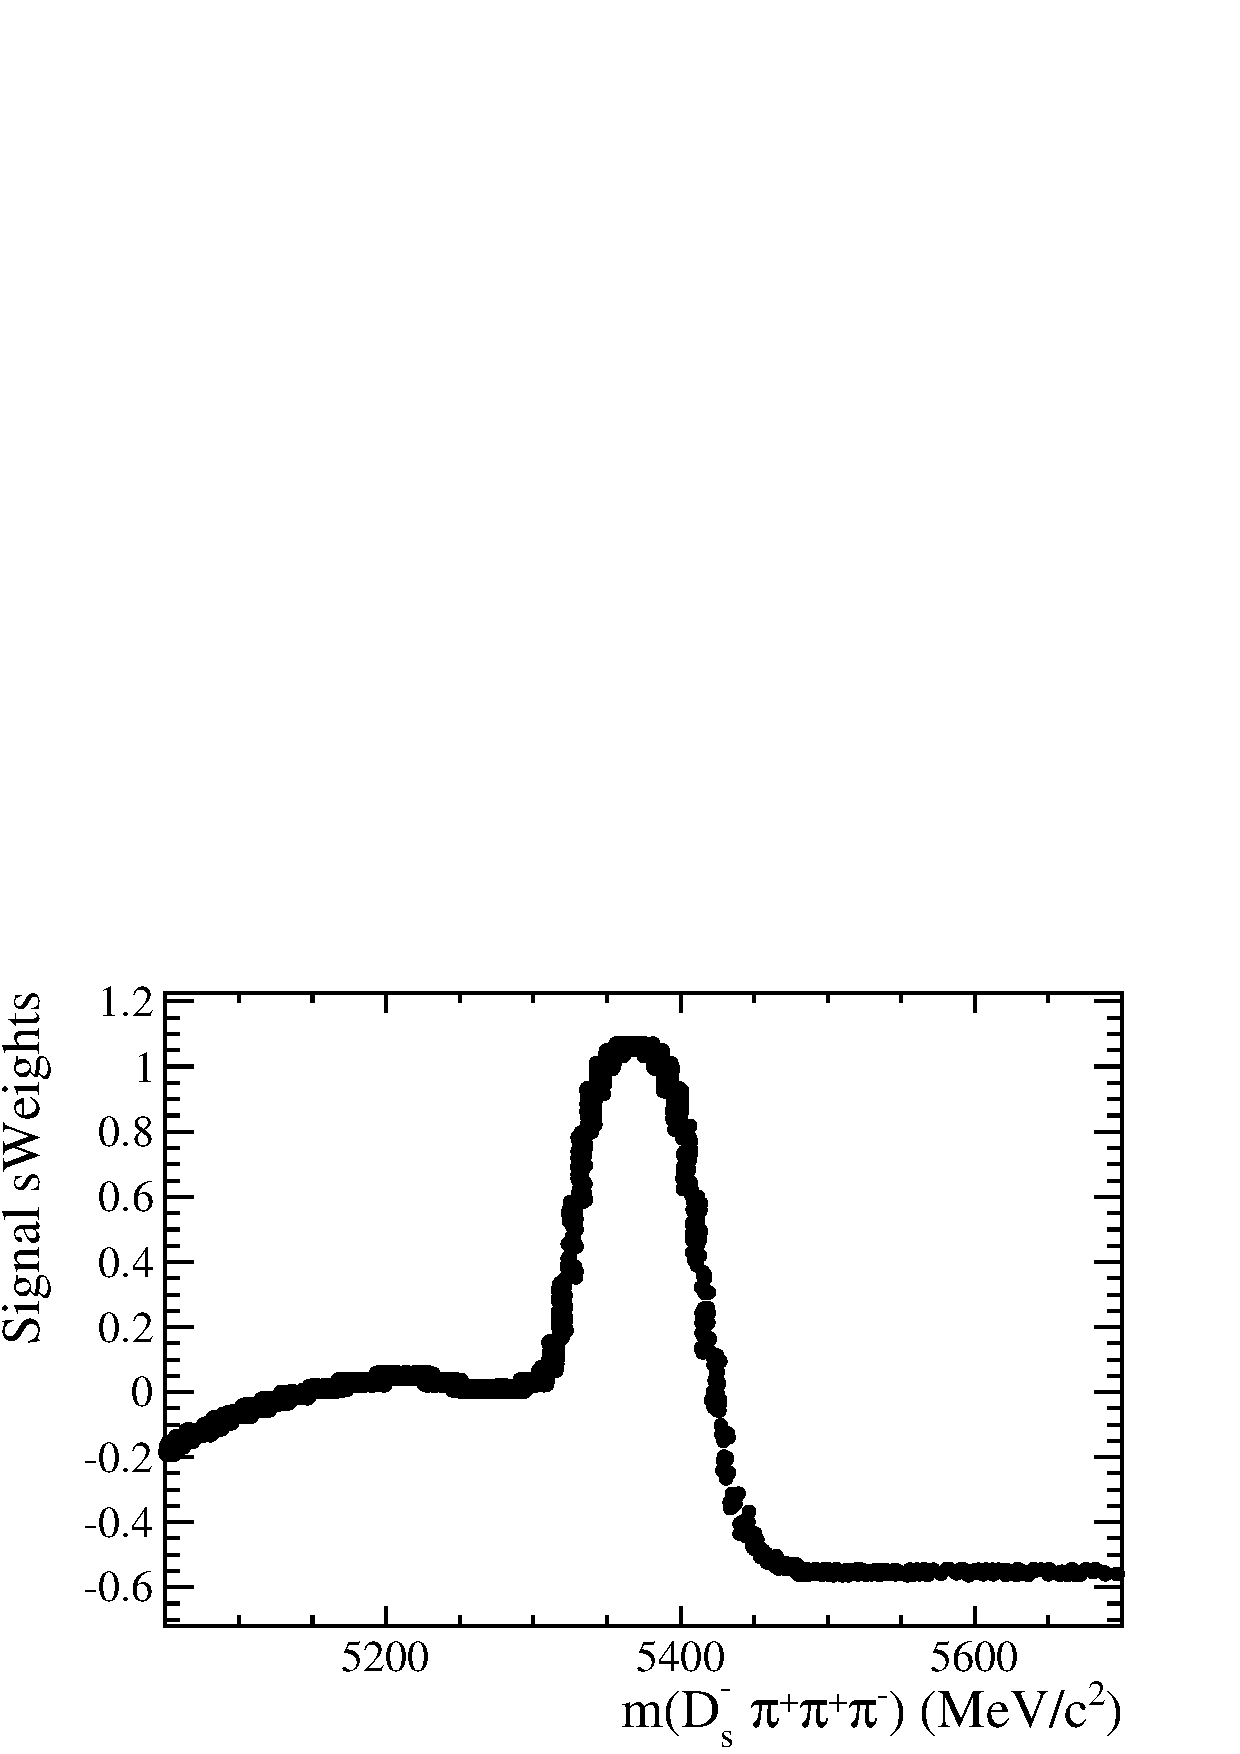
\includegraphics[height=7.cm,width=0.49\textwidth]{figs/norm_sweight_y11_phipi.pdf}
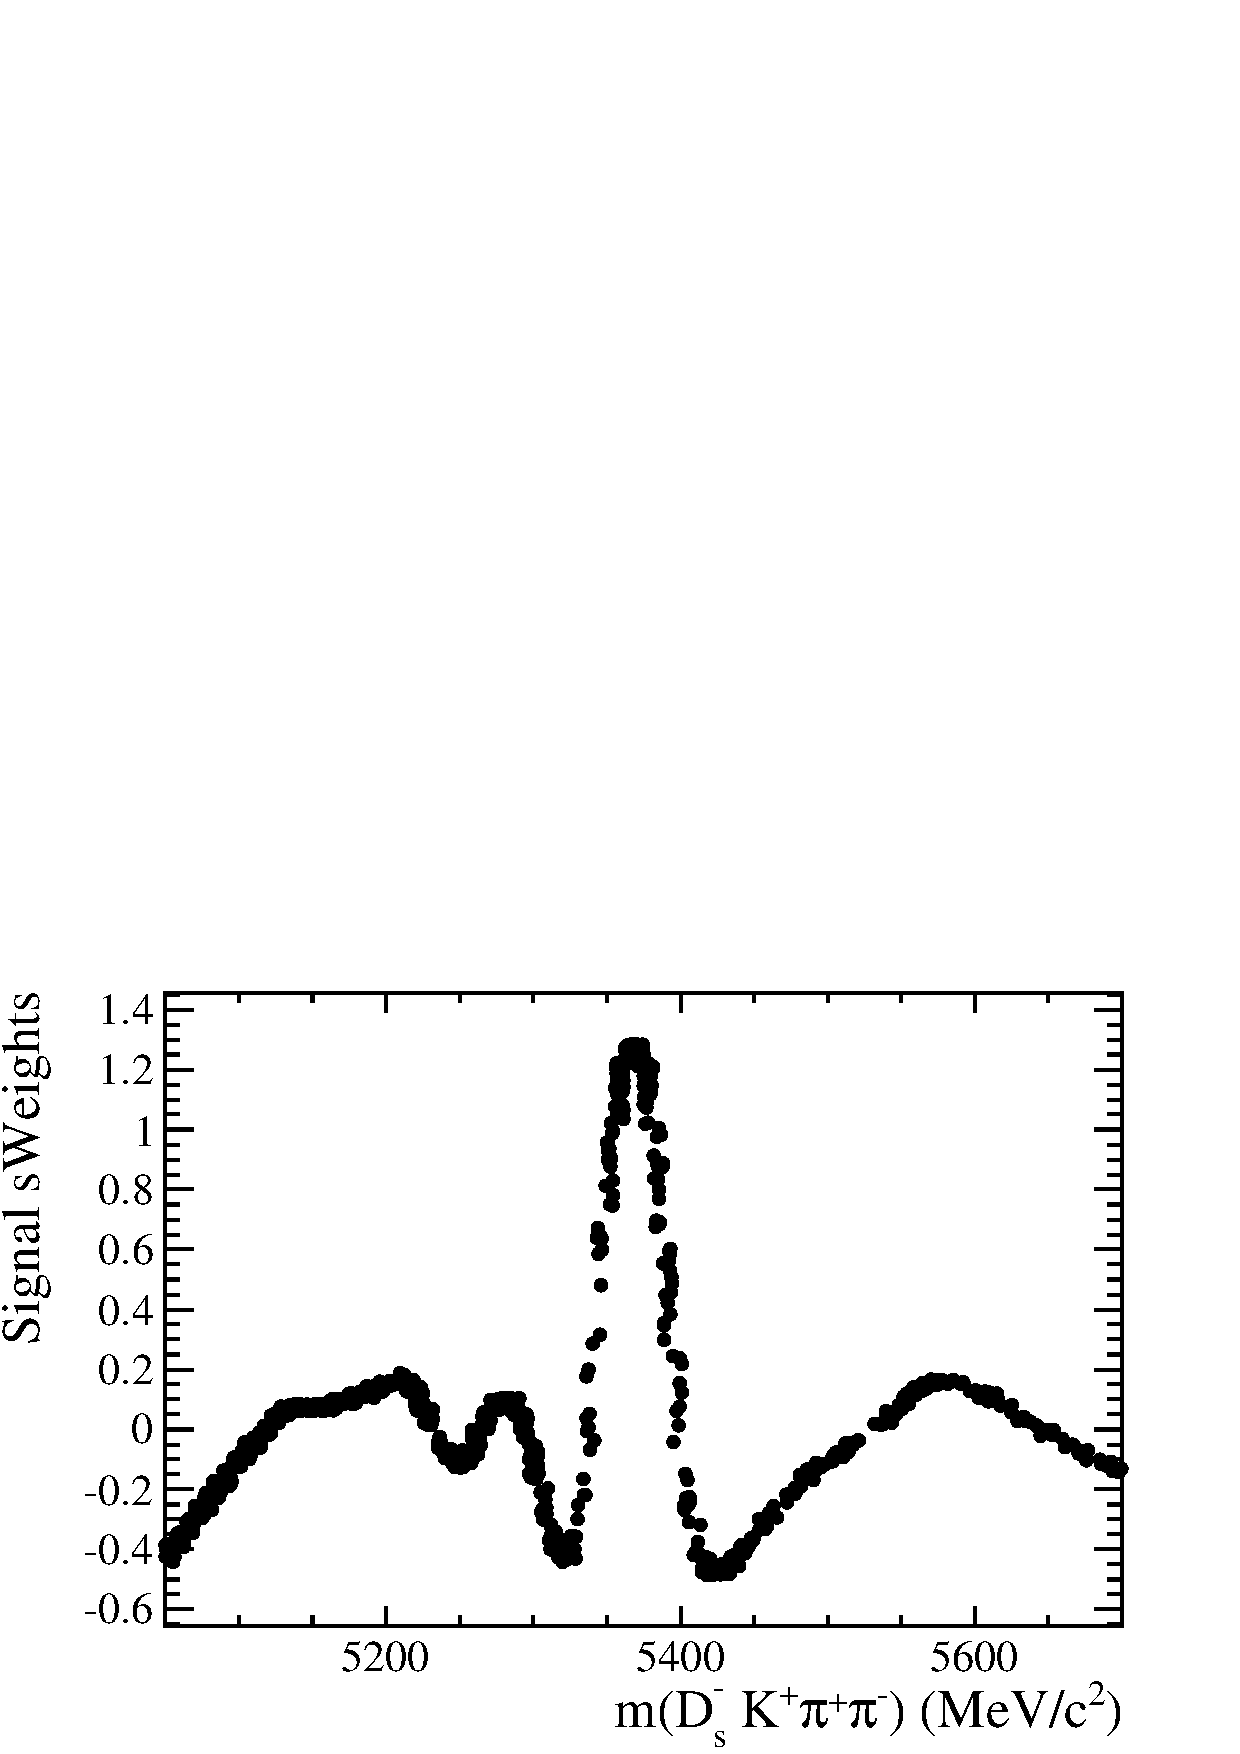
\includegraphics[height=7.cm,width=0.49\textwidth]{figs/signal_sweight_y11_phipi.pdf}
\caption{Distribution of sWeights across the invariant mass of (left) $\Bs\to\Ds\pion\pion\pion$ and (right) $\Bs\to\Ds\kaon\pion\pion$ candidates for Run1 and Run2 data.}
\label{fig: sWeights}
\end{figure}
